\section{Other cryptographic tasks}
\label{sec:other}

In our description so far we have adopted the composable view and
regarded cryptographic protocols as constructions, i.e., protocols
construct some resources given other resources.\footnote{See also
  Footnote~\ref{fn:resourcetheory} for other uses of resource theories
  in quantum mechanics.} Cryptographic protocols proposed in the
literature have not always been defined in this way, but instead are
specified in terms of particular security\-/like properties, e.g.,
that an adversary is unable to guess the content of an encrypted
message. Sometimes these properties can be rephrased as an ideal
system within the real\-/world ideal\-/world paradigm, as discussed in
\secref{sec:qkd.other.ac}. In this section we review some of the major
results in quantum cryptography from this perspective, i.e., we
present them as constructive statements, defining the resources
constructed and used by the protocols. For a broader review of quantum
cryptography, we refer to a recent survey by \textcite{BS16}.


\subsection{Secure quantum message transmission}
\label{sec:qmt}

From a theory of resources perspective, the task of securely
transmitting a quantum message from Alice to Bob is nearly identical
to the corresponding classical task, analyzed in \secref{sec:smt}. Here too, we
require the players to share a secret key resource and an insecure
channel, and the goal is to construct a secure channel \--- the only
difference being that the insecure and secure channels are both
quantum channels. We have already encountered insecure quantum
channels in \secref{sec:qkd}, where they were used for QKD. A secure
quantum channel is modeled analogously to a secure classical channel
as drawn in \figref{fig:secure.resource}, except that the messages
sent are quantum. We depict this in
\figref{fig:secure.quantum.resource}.

\begin{figure}[tb]

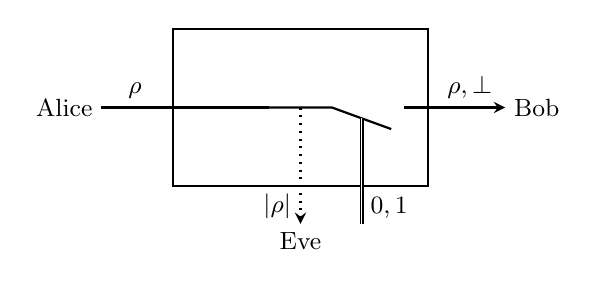
\begin{tikzpicture}[
sArrow/.style={->,>=stealth,thick},
largeResource/.style={draw,thick,minimum width=1.618*2cm,minimum height=2cm}]

\small

\def\z{.4}

\node[largeResource] (keyBox) at (0,0) {};
\node (alice) at (-3,0) {Alice};
\node (bob) at (3,0) {Bob};
\node (eve) at (0,-1.7) {Eve};
\node (juncLL) at (-3*\z,0) {};
\node (juncLR) at (-\z,0) {};
\node (juncRL) at (\z,0) {};
\node (juncRR) at (3*\z,0) {};

% \draw[thick] (alice) to node[pos=.35,auto] {$\rho$} (juncLL.center) to node[pos=.5]
% (handle1) {} +(340:2*\z);
\draw[thick] (alice) to node[pos=.2,auto] {$\rho$} (juncLR.center);
\draw[thick] (juncLR.center) to (juncRL.center) to node[pos=.5]
(handle2) {} +(340:2*\z);
\draw[sArrow] (juncRR) to node[pos=.65,auto] {$\rho,\bot$} (bob);
\draw[sArrow,dotted] (0,0) to node[pos=.85,auto,swap] {$|\rho|$} (eve);
% \draw[double] (handle1.center |- eve.north) to node[pos=.15,auto,swap] {$0,1$} (handle1.center);
\draw[double] (handle2.center |- eve.north) to node[pos=.15,auto,swap] {$0,1$} (handle2.center);

\end{tikzpicture}

\caption[Secure quantum channel]{\label{fig:secure.quantum.resource}A
  secure quantum channel that allows Eve to learn the length of the
  quantum message \--- informally denoted as $|\rho|$ \--- and prevent
  Bob from receiving it: when Alice inputs a message $\rho$ at her
  interface, information about the length of the message is given to
  Eve, who can additional press a switch that either delivers Alice's
  message to Bob or provides him with an error message $\bot$
  instead.}
\end{figure}

The first protocols that construct such a secure quantum channel from a shared secret key and an insecure channel were proposed by \textcite{BCGST02}. They follow the same pattern as classical message transmission: one first encrypts the quantum message with a quantum OTP, then encodes it in a larger space so as to detect any errors that may be introduced by an adversary. However, contrary to the case of classical messages, there is no known way to view these two steps as two distinctive constructive statements, i.e., as a construction of an authentic channel from an insecure channel, and a second construction of a secure channel from an authentic channel. This means that the analysis has to include both aspects at the same time.

In \secref{sec:qmt.protocol} we explain this construction and in
\secref{sec:qmt.related} we review additional work on the topic. At
the end of this section, in \secref{sec:computational}, we 
revisit this topic from a computational perspective.

\subsubsection{Generic protocol}
\label{sec:qmt.protocol}

The classical OTP introduced in \secref{sec:ac.otp} can be seen as
randomly flipping each bit of the message. The quantum OTP
\cite{AMTW00,BR03} follows the same principle: one flips the bits and
phases of the message at random. For $x,z \in \{0,1\}^n$, let $X^x$
and $Z^z$ denote operators on $\left(\complex^2\right)^{\otimes n}$
which perform bit and phase flips in positions indicated by the
strings $x$ and $z$, respectively. The quantum OTP consists of
choosing $x$ and $z$ uniformly at random, and applying the
corresponding operation to the message. For any state $\rho_{MR}$
where $M$ is a register of size $2^n$, we thus have
\[ 
\frac{1}{2^{2n}}\sum_{x,z} Z^z X^x \rho_{MR} X^x Z^z = \tau_M
\otimes \rho_R,
\]
where $\tau_M$ is the fully mixed state and $\rho_R$ is the reduced
density operator of $\rho_{MR}$. We call the operators $Z^zX^x$
defined this way \emph{Pauli operators}.\footnote{This notation
  simplifies the presentation here, but deviates from the more
  commonly used definition of the Pauli operators as
  $i^{z \cdot x} Z^z X^x$, where $z \cdot x = \sum_j z_jx_j$ and $i$
  is the imaginary unit.}

The second ingredient needed to construct a secure quantum channel is
an error correcting code that is going to be used to detect errors in
the transmission, i.e., tampering by an adversary. Generally, an error
correcting code may be seen as a map from a message space $\hilbert_M$
to a larger (physical) space $\hilbert_C$. For simplicity, we model
the encoding for a code $\cC_k$ as first appending a state
$\ket{0} \in \hilbert_T$ to the message $\rho_M$, where
$\hilbert_C = \hilbert_M \otimes \hilbert_T$, followed by applying a
unitary $U_k$ to the resulting state, e.g.,
$\sigma_{C} = U_k \left( \rho_M \otimes \proj{0} \right)
\hconj{U}_k$.

To test whether an error occurred, one decodes the received state
$\tilde{\sigma}_{C}$ by applying the inverse operation $\hconj{U}_k$
and measures the $T$ register in the computational basis. If the
result is not $0$, then this is evidence for noise. We say that a code
detects an error $V$ if after decoding a message to which this error
was applied \--- i.e., $\tilde{\sigma}_{C} = V \sigma_{C} \hconj{V}$
\--- one always gets a measurement outcome different from
$0$. Furthermore, we call an error \emph{trivial} if it never affects
the code word, i.e., for any $\rho_M$,
\[ 
  \hconj{U}_k V U_k \left( \rho_M \otimes \proj{0} \right)
\hconj{U}_k \hconj{V} U_k = \rho_M \otimes \proj{0}.
\]

For an error $V$ to modify a message and yet not be caught, it must be
non-trivial and not detected by the code used. For the purpose of
constructing a secure channel according to the method of
\textcite{BCGST02}, it is sufficient to detect all Pauli
errors. \textcite{BCGST02} define a set of codes, which they call
\emph{purity testing codes}. They guarantee that with high probability
over the choice of code, all Pauli errors are either caught or
trivial. More precisely, a set $\{\cC_k\}_k$ of codes forms a family
of $\eps$\=/purity testing codes if, for any Pauli error $X^xZ^z$, the
probability over a uniformly random choice of $k$ that this error is
neither caught nor trivial is less than $\eps$.

The protocol for constructing a secure channel then works as
follows. The sender first encrypts the message with a quantum OTP,
i.e., a Pauli operator $Z^zX^x$ chosen uniformly at random according
to the secret key. Then a state $\ket{s}$ is appended to the message,
where $s$ is also chosen uniformly at random according to the
key. Finally, the resulting state is encoded with a unitary $U_k$
corresponding to the encoding operation of an element of a purity
testing code family $\{\cC_{k}\}_{k}$, where again $k$ is chosen
uniformly at random according to the secret key. Decryption works in
the obvious way: the receiver applies the inverse operator
$\hconj{U}_k$ and then measures the $T$ register. If the outcome is
not $s$, the message was jumbled and the player outputs an error
symbol. Otherwise, the receiver decrypts the message with the operator
$Z^zX^x$.

\subsubsection{Concrete schemes}
\label{sec:qmt.related}


\textcite{BCGST02} introduced the general family of protocols
described in \secref{sec:qmt.protocol}, and also provided a concrete
construction of a purity testing code family that has good
parameters. Following this seminal work, a variety of further
protocols for authentication of quantum messages have been proposed in
the literature, which are based on different codes. Authentication
using the signed polynomial code \cite{BCGHS06,ABE10}, the trap code
\cite{BGS13,BW16}, the Clifford code \cite{ABE10,DNS12,BW16} \---
which is a unitary $3$\-/design~\cite{Web15,Zhu17} \--- a unitary
$8$\-/design \cite{GYZ17} and a unitary $2$\-/design\footnote{Because
  any unitary $t$\-/design for $t \geq 2$ is a unitary $2$\-/design,
  it follows that any $t$\-/design constructs a secure quantum
  channel.}  \cite{Por17,AM17} are all instances of the family from
\textcite{BCGST02}, with alternative purity testing
codes.\footnote{Most of these works consider a construction where the
  message is first encoded with a purity testing code, and then
  encrypted. But as shown in \textcite{Por17}, this is equivalent to
  the original scheme of \textcite{BCGST02}, which reverses the order
  of these two operations.} To the best of our knowledge, only the
Auth-QFT-Auth scheme from \textcite{GYZ17} is not known to follow the
model of \textcite{BCGST02}.

Although most of these works provide some kind of security proof for
the protocol, only two papers consider a composable security
definition, namely \textcite{HLM11,Por17}. Both works show that the
family of protocols from \textcite{BCGST02} construct a secure quantum
channel from a shared secret key and an insecure quantum channel. It
should be noted however that \textcite{HLM11} considers a restricted
class of distinguishers \--- those that perform a substitution attack
(see \secref{sec:smt.auth}) \--- and \textcite{Por17} only analyzes a
subset of this family, for which the purity testing code family
detects all (rather than only non-trivial) errors with high
probability.\footnote{One refers to this as a \emph{strong} purity
  testing codes.} In fact both papers prove that one may additionally
recycle part of the key, which is discussed further in the following
section.


\subsection{Key reuse in classical and quantum message transmission}
\label{sec:recycle}

As already mentioned in Secs.~\ref{sec:smt.auth} and
\ref{sec:qmt.related}, part of the key used in the constructions of
secure channels may be recycled, i.e., at the end of the protocol it
can be added back to a pool of secret key bits. For example, in the
case of classical message authentication analyzed in
\secref{sec:smt.auth}, the sender appends a tag $y = h_k(x)$ to the
message $x$. The value of the tag $y$ depends on the shared secret key
$k$, and every bit of the tag leaks (at most) a bit of the secret key
to the adversary. But the key is longer than the tag, so the bits
which are not leaked may be reused. It is however vital that they are
not recycled too soon: if the sender reuses part of the key before the
receiver obtains the (authenticated) message, the adversary may learn
these bits and use this information to successfully change the message
and authentication tag.

To recycle key bits in classical or quantum message transmission, the
real system is changed as follows. Firstly, the players need an extra
resource, a $1$-bit backwards authentic channel, allowing the receiver
to tell the sender whether the message was successfully received or
not. Once this confirmation is sent, the receiver may recycle part of
the key, i.e., it is output by the corresponding converter. And once
this confirmation is received by the sender, she also recycles the
same part of the key. The ideal resource constructed in this way
corresponds to the parallel composition of a secure (or authentic)
channel and a secret key resource, drawn in
\figref{fig:keyrecycle.ideal}. As previously, the adversary may
control whether the message is delivered on the secure channel. And
since the amount of key recycled may depend on the adversary's
behavior as well---namely by allowing or preventing the message from
being delivered, we model the resource as being equipped with a switch
to control how much key the players get.

\begin{figure}[tb]


\begin{tikzpicture}[
sArrow/.style={->,>=stealth,thick},
thinResource/.style={draw,thick,minimum width=3.2cm,minimum height=1cm}]

\small

\def\t{2.5} %.9+1.6
\def\v{.8}
\def\e{2.2} %.8+.5+.9
\def\z{.4}

\node (a1) at (-\t,\v) {};
\node (a2) at (-\t,-\v) {};
\node (b1) at (\t,\v) {};
\node (b2) at (\t,-\v) {};
\node (eve) at (0,-\e) {};

\node[thinResource] (keyBox) at (0,\v) {};
\node[draw] (key) at (0,\v) {key};
\node[yshift=0,above right] (keyname) at (keyBox.north west) {\footnotesize
  Secret key $\aK$};

\draw[sArrow] (key) to node[auto,swap,pos=.85] {$k$} (a1);
\draw[sArrow] (key) to node[auto,pos=.85] {$k$} (b1);
\draw[double] (eve.center) to node[pos=.08,auto,swap] {$0,1$} (key);

\node[thinResource] (channel) at (0,-\v) {};

\node (juncLL) at (-3*\z,-\v) {};
\node (juncLR) at (-\z,-\v) {};
\node (juncRL) at (\z,-\v) {};
\node (juncRR) at (3*\z,-\v) {};

% \draw[thick] (alice) to node[pos=.35,auto] {$\rho$} (juncLL.center) to node[pos=.5]
% (handle1) {} +(340:2*\z);
\draw[thick] (a2) to node[pos=.15,auto] {$\rho$} (juncLR.center);
\draw[thick] (juncLR.center) to (juncRL.center) to node[pos=.5]
(handle2) {} +(340:2*\z);
\draw[sArrow] (juncRR) to node[pos=.6,auto] {$\rho,\bot$} (b2);
\draw[sArrow,dotted] (-2*\z,-\v) to node[pos=.8,auto,swap] {$|\rho|$}
(-2*\z,-\v |- eve.center);
% \draw[double] (handle1.center |- eve.north) to node[pos=.15,auto,swap] {$0,1$} (handle1.center);
\draw[double] (handle2.center |- eve.center) to node[pos=.2,auto,swap] {$0,1$} (handle2.center);

\node[yshift=0,above right] at (channel.north west) {\footnotesize
  Secure channel $\aS$};

\node[inner sep=0] (justadot) at (0,1.5) {};

\node[draw,thick,dashed,fit=(channel)(keyBox)(justadot),inner sep=8] (alltogether) {};



\end{tikzpicture}


\caption[Ideal secure channel with
key]{\label{fig:keyrecycle.ideal}The ideal system for a secure channel
  with key recycling: it consists of a secure channel $\aS$ and key
  resource $\aK$. The adversary controls the length of the 
  recycled key (through her input to $\aK$) as well as whether the
  receiver obtains the message (through her input to $\aS$).}
\end{figure}

In the case of authentication of classical messages, \textcite{WC81}
already proposed that part of the key can be safely recycled. Here, if
the $2$-universal hash function has the special form
$h_{k_1,k_2}(x) = {f_{k_1}(x) \xor k_2}$, where $k_2$ is a bit string
of the same length as the tag, then $k_1$ may be recycled, but a new
$k_2$ is needed for every message. It was proven by \textcite{Por14}
that this scheme is composable and constructs the ideal resource
described above.

In the case of quantum messages, roughly the same holds in the case
where the message fails the authentication: the number of bits of key
leaked depend on the length of the ciphertext and the rest can be
recycled.\footnote{If the ciphertext is $n$ qubits long, about $2n$
  bits of key are lost, see \textcite{Por17} for the exact
  parameters.} But in the case where the message is accepted, the
players can recycle more key. This holds because of the no\-/cloning
principle of quantum mechanics: if the receiver holds the correct
ciphertext, then the adversary cannot have a copy of it, and thus does
not hold any information about the key either. It was first shown by
\textcite{HLM11} that nearly all of the key could be recycled in the
case where the message is accepted. Then \textcite{Por17} showed that
every bit of the key can indeed be recycled. This is not known to hold
for all schemes that construct a secure quantum channel, but so far
only for those that use strong purity testing codes \cite{Por17}.

\subsection{Delegated quantum computation}
\label{sec:dqc}

The setting in which a client, typically with bounded computational
resources, asks a server to perform some computation for her is called
\emph{delegated computation}. The client might not want the server to
learn what computation it is performing for her, and wish to run a
protocol that hides the underlying computation \--- this property is
called \emph{blindness} in the literature. Furthermore, the client
might want to verify that the server correctly performed the
computation she required \--- this is known as \emph{verifiability}.

The task of delegating a quantum computation was first studied by
\textcite{Chi05}, with the goal of achieving blindness. In follow-up
works, the requirements on the client's information-processing
abilities were reduced. \textcite{BFK09} proposed the first protocol
for blind delegated quantum computation that does not require the
client to have quantum memory, but only the ability to prepare
different pure states. This result was extended in \textcite{FK17} to
include verifiability as well.

Delegated quantum computation (DQC) was formalized as a constructive
statement by \textcite{DFPR14}. The authors modeled a DQC protocol
that achieves both blindness and verifiability as constructing a
resource $\aS^{\blind}_{\verif}$ that works as follows. It first
receives a description of the required computation as a state $\psi$
from the client. Every computation necessarily leaks some information
to the server, e.g., an upper bound on the computation size, so the
resource computes this leaked information $\ell$ and outputs it at the
server's interface. The server can then decide if it will cheat \---
in which case the client will however get an error message \--- or
output the correct result of the computation, which is evaluated by
applying an operator $\cU$ to the input. This is depicted in
\figref{fig:dqc.ideal}. A DQC protocol constructs such a resource from
nothing more than a shared communication channel between client and
server.

\begin{figure}[tb]

\begin{tikzpicture}[
sArrow/.style={->,>=stealth,thick},
blocResource/.style={draw,minimum width=4cm,minimum height=1.9cm},
brnode/.style={minimum width=3.4cm,minimum height=.2cm}]


\small

\def\u{2.75}%4/2+.75 
\def\v{.6}

\node[brnode] (n1) at (0,\v) {};
%\node[brnode] (n2) at (0,0) {};
\node[brnode] (n3) at (0,-\v) {};
\node[blocResource] (S) at (0,0) {};
\node[yshift=-1.5,above right] at (S.north west) {{\footnotesize
  Secure DQC resource} $\aS^{\blind}_{\verif}$};
\node[text width=3.3cm] at (0,.1) {\footnotesize
  \begin{align*}
   \psi^\ell & = \Pi_\ell \psi \Pi_\ell, \\
   \rho^\ell & = \begin{cases}
    \cU(\psi^\ell) \text{ if $c=0$,} \\ \proj{\err}
    \text{ if $c=1$.} \end{cases} \end{align*}};

\node (a1) at (-\u,\v) {};
\node (a3) at (-\u,-\v) {};
\node (b1) at (\u,\v) {};
%\node (b2) at (\u,0) {};
\node (b3) at (\u,-\v) {};

\draw[sArrow] (a1.center) to node[auto,pos=.4] {$\psi$} (n1);
\draw[sArrow] (n3) to node[auto,swap,pos=.6] {$\rho$} (a3.center);

%\draw[sArrow,double] (b1.center) to node[auto,swap,pos=.4] {$b$} (n1);
\draw[sArrow] (n1) to node[auto,pos=.6] {$\ell$} (b1.center);
\draw[sArrow,double] (b3.center) to node[auto,swap,pos=.4] {$c$} (n3);

\end{tikzpicture}

\caption[Ideal DQC resources]{\label{fig:dqc.ideal}Ideal DQC
  resource. The client has access to the left interface, and the
  server to the right interface. The server obtains some information
  $\ell$ about the input, and can decide if the client gets the
  correct outcome or an error by inputting a bit $c$.}
\end{figure}

A weaker resource that provides only blindness but not verifiability
can be obtained by increasing the power of the server at its interface
of the resource: instead of inputing a bit that decides if the client
gets the correct outcome, the server can decide what output the client
gets, but still only receives the leaked information $\ell$
\cite{DFPR14}.

In \textcite{DFPR14} the protocols from \textcite{BFK09,FK17} were
shown to satisfy the corresponding constructive definitions. These
protocols still require the client to prepare a few different single
qubit quantum states and send them to the server. In order to better
analyze this requirement, \textcite{DK16} decomposed the construction
of a DQC resource in two steps. First, they consider a resource which
provides the server with the random states it needs (and the client
with a description of which state was given to the server), then the
DQC protocol constructs the DQC resource given this state preparation
resource. This decomposition then allowed \textcite{GV19} to design a
protocol that constructs the required state preparation resource for
an entirely classical client \--- this was achieved by sacrificing
information\-/theoretic security for computational security. Composing
this with a DQC protocol, one gets DQC for an entirely classical
client, albeit with computational security. This is believed not to be
possible with information\-/theoretic security~\cite{ACGK19}. We note
however that \textcite{GV19} make a non\-/standard assumption about
available resources, without which such a result does not seem
possible \cite{BCCKLMW20}.

It is instructive to compare this to early definitions of blindness,
e.g., those from \textcite{BFK09,FK17}. There, the requirement is that
the server learns nothing about the computation except for the allowed
leaked information $\ell$. Roughly speaking, this means that the state
$\rho^{\psi^\ell}$ held by the server at the end of the protocol \---
where $\psi^\ell$ is an input that leaks information $\ell$ \--- must
be such that \begin{equation}\label{eq:dqc.standalone}
  \rho^{\psi^\ell} \approx \rho^\ell,\end{equation} i.e., it can only
depend on $\ell$, but not on any other part of the input. If we
compare this to the constructive definition from \textcite{DFPR14}, in
which the distinguisher has access to both the server's interface and
the client's interface of the resources, \eqnref{eq:dqc.standalone}
corresponds to the special case where we do not maximize over all
distinguishers, but only those that ignore the output received by the
client. Following \secref{sec:qkd.other.ac} one may express this as a
restriction on the resource constructed instead of a restriction on
the distinguisher: requiring a DQC protocol to satisfy
\eqnref{eq:dqc.standalone} is (mathematically) equivalent to requiring
it to construct an ideal resource that does not provide the client
with the result of the computation.
%Alternatively, one can capture this condition if the protocol
% and ideal resource are restricted so as not to provide the client with
% an output. This is however a rather pointless resource that is
% constructed by such a security definition, since if the client is not
% going to receive any output, she should not run the protocol in the
% first place.

\subsection{Multi-party computation}
\label{sec:mpc}

In this section we consider a setting where multiple mutually
distrustful parties wish to evaluate a (possibly randomized) function
to which each of them provides an input \--- or they wish to jointly
evaluate a CPTP map on shared quantum inputs. They however do not want
the other parties to learn anything about their input other than
what can be learnt from the output. Furthermore, they also want to
guarantee that if they get an output, then this is the correct
output. An example is a function that outputs which player $i$ has the
largest input $x_i$ \--- e.g., the players want to know who earns more
without revealing their salary to the others. Another example is
generating a random coin flip, in which case no input is
required. Generally speaking, multi-party computation corresponds to constructing an ideal resource
which first takes the inputs from all parties and then provides them
with the correct output.

\subsubsection{Bit commitment}
\label{sec:mpc.BC}

A bit commitment resource is a system in a two-party setting, which
forces a player (say, Alice) to commit to a value, but without
revealing this value to the other player (say, Bob). At some later
point, the commitment is ``opened'', so that Bob may know to what
value Alice committed. More precisely, Alice sends a bit $b$ to the
resource, and Bob is notified that Alice is committed to a
value. Alice may then send an open command to the resource, at which
point $b$ is delivered to Bob. In the classical setting, such a
resource cannot be constructed from communication channels
alone~\cite{CF01,MR11}, but extra resources such as a common reference
string \--- a random string shared by all parties \--- are
needed~\cite{CF01}.

The argument from \textcite{MR11} has been extended in
\textcite{VPdR19} to prove that even if the players use quantum
protocols and even if the adversary is computationally bounded, has
only bounded or noisy storage and is restricted by relativistic
constraints,\footnote{This means that the adversary cannot send
  information between two points faster than light takes to travel
  between the two points, see \secref{sec:relativistic}.} it is still
impossible to construct a bit commitment resource without further
setup assumptions than communication channels.

It has been suggested that one could construct bit commitment if one
takes relativity into account, i.e., that messages cannot be sent
faster than the speed of light \cite{Ken99,Ken12,KTHW13}. However,
these protocols do not construct a bit commitment resource:
\textcite[Appendix A]{Kan15}\footnote{The proof from
  \textcite[Appendix A]{Kan15} uses the same attack as
  \textcite{BCMS98}, where it is shown that some non\-/composable
  definitions of bit commitment appearing the classical literature
  cannot be used to force a quantum player to commit to a measurement
  outcome.} proves that if one composes these relativistic bit
commitment protocols with the protocol from \textcite{Unr10} to
construct oblivious transfer from bit
commitment,\footnote{\emph{Oblivious transfer} and the construction
  from \textcite{Unr10} are discussed in \secref{sec:mpc.OT}.} then
the result is not a secure oblivious transfer protocol. It has now
been proven that taking relativity into account is not sufficient to
achieve bit commitment \cite{VPdR19}, which we discuss in more detail
in \secref{sec:relativistic}.

\subsubsection{Coin flipping}
\label{sec:mpc.CF}

Another well studied resource is that of coin flipping, which flips a
random coin and provides both players with the result. The
impossibility proof for bit commitment from \textcite{MR11} can be
adapted to show that coin flipping and biased coin flipping (where a
player is allowed to partially bias the flip) are also impossible
without further assumptions.  Note that this proof is valid
independently of whether one considers classical or quantum
strategies. A direct proof for the impossibility of coin flip in the
quantum and relativistic setting \--- even in the case of
computational- and memory\-/bounded adversaries \--- is given in
\textcite{VPdR19}.

\emph{Coin expansion} is a weaker task, in which one constructs a
resource that produces a sequence of coin flips from a weaker resource
that produces fewer coin flips. This has been shown to be impossible
for classical players with information\-/security \cite{HMU06,SM16},
but is possible with computational security \cite{HMU06} and remains
open in the quantum case.

% Classically one can construct (biased) coin flips from bit commitment
% \cite{Blu83,DM13}. So the impossibility proof for (biased) coin flips
% \cite{MR11,VPdR19} immediately implies that it is also impossible to
% construct a bit commitment resource in the quantum setting.


\subsubsection{Two-party function evaluation and oblivious transfer}
\label{sec:mpc.OT}

It has been shown by \textcite{IPS08} that a resource that evaluates
any classical probabilistic polynomial\-/time function with two inputs
can be constructed given an \emph{oblivious transfer} resource, i.e.,
a system that receives two strings $s_0,s_1$ from one player, Alice, a
bit $c$ from the second player, Bob, and sends Bob $s_c$.

In the quantum setting, it is possible to construct an oblivious
transfer resource from a \emph{bit commitment} resource. The
construction of oblivious transfer from bit commitment was first
proposed by \textcite{CK88}, adapted to noisy channels in
\textcite{BBCS92}, and proven secure by \textcite{Unr10}. Combining
this result with \textcite{IPS08}, it follows that bit commitment is
universal for classical two-party computation \cite{Unr10}.

It is however not possible to construct an oblivious transfer resource
from nothing but communication channels, even if the adversary is
computationally bounded, has only bounded or noisy storage and is
restricted by relativistic constraints~\cite{LdR21}.

\subsubsection{Everlasting security}
\label{sec:mpc.ever}

\textcite{Unr13} studied multi-party computation in the setting of
\emph{everlasting security}. This means that one relies upon a
computational assumption, but this assumption has to be broken
\emph{during} the execution of the protocol for an adversary to break
the scheme. If this is not the case, then even a computationally
unbounded adversary cannot get any significant advantage after the
protocol has terminated. This is generally not satisfied by
computational encryption schemes, because an adversary could obtain a
ciphertext and wait for an advancement in algorithms to break the
scheme and obtain the message. But if a computational authentication
scheme is executed, then the adversary must be able to perform the
hard computation before the message is received and authenticated.

Composition in such a setting is not straightforward, and
\textcite{Unr13} provides the necessary definition a scheme must
satisfy to be composable. They show how to perform
authentication given a signature card, which, when composed with QKD
and secure encryption as in \secref{sec:smt}, results in a secure
channel. They also provide a way to perform bit commitment based on signature
cards. Composing this with the protocols from \secref{sec:mpc.OT}
allows one to perform any multi-party computation with everlasting
security.

\subsubsection{Multi-party quantum computation}
\label{sec:mpc.MPQC}

The tasks studied so far in this section are concerned with
multi-party evaluation of a classical function \--- so\-/called
multi-party computation (MPC) \--- but using quantum communication and
computation to possibly achieve what cannot be done classically. The
problem of multi-party \emph{quantum} computation (MPQC) generalises this to the case where the
inputs and outputs are quantum \cite{CGS02,BCGHS06,DNS12,DGJMS20,LRW20,ACCHLS21}. The relation between inputs and outputs is then most generally described by a CPTP. It is standard to
use a composable framework for analyzing classical MPC
\cite{CDN15}. But to the best of our knowlege, the only work on MPQC
that mentions that the results hold in a composable framework is
\textcite{BCGHS06} \--- and they only provide a proof sketch. All
other works assume that the dishonest party performs their attack in
an isolated way, only interacting with the environment (the
distinguisher) before the protocol starts and after the protocol
ends. This is the so\-/called \emph{stand\-/alone} security model, and
protocols proven secure in such a model do not necessarily compose
concurrently with other protocols, in particular, they might not be
secure if two instances of the same protocol are run in
parallel. Nonetheless, for MPQC we do not know of any
attacks on protocols run concurrently, and it is plausible that
exactly the same result go through in a composable security framework.

The ideal resource one wishes to construct in MPQC receives the inputs
from all parties, performs the quantum computation, and then provides
each player with their part of the output. The works of
\textcite{CGS02,BCGHS06,LRW20} consider an ideal resource which is
guaranteed to provide the output to the honest
players. \textcite{CGS02} first show that this can be achieved if the
fraction of dishonest parties is $t < n/6$, where $n$ is the total
number of players. In \textcite{BCGHS06} this is improved to $t < n/2$
cheating parties. \textcite{LRW20} decrease the number of qubits and
communication complexity needed to get the same.

In \textcite{DNS12,DGJMS20,ACCHLS21} the ideal resource is defined
such that it first provides the dishonest parties with their share of
the output. They then provide a bit to the ideal resource, which
indicates whether the honest parties should also receive their output
or an abort symbol instead. This is called
\emph{unfairness}. Weakening the ideal resource in this way allows the
number of dishonest parties to be any $t < n$. \textcite{DNS12} first
show how to do this in the two-party case. \textcite{DGJMS20} extend
this to the multi\-/party setting.  \textcite{ACCHLS21} improve the
protocol to identify parties that abort, so that if an abort occurs,
the faulty party can be excluded and the others start again without
them.

We note that all these protocols assume that classical MPC is
available as a resource \--- usually, for the same
number of dishonest players and the same abort conditions as the
constructed MPQC. So all these results require the same setup
assumptions as the corresponding classical MPC. For example, for
$t < n/3$ and guaranteed output one can do classical MPC assuming only
pairwise secure channels between the players~\cite{CDN15}. For
$t < n/2$ and guaranteed output one additionally needs broadcast for
information\-/theoretic security, but pairwise authentic channels are
sufficient for computational security~\cite{CDN15}. If we drop
fairness, then in the case of computational security one gets unfair
security for any $t < n$ if one assumes oblivious transfer \cite{GMW87} or
a common reference string \cite{CLOS02}, and information\-/theoretic
security if one assumes common shared randomness \cite{IOZ14}.


\subsubsection{One-time programs}
\label{sec:mpc.OTP}

A special class of multi-party functionalities that have been studied
in more detail are non\-/reactive, sender\-/oblivious functions, i.e.,
one player is labeled ``sender'', another ``receiver'', and only the
receiver obtains the output of the function. This special structure
allows for non\-/interactive protocols to construct a resource that
computes such a function: communication goes only from the sender to
the receiver. The receiver can use the information obtained to
evaluate the function on one input. But by definition of the ideal
resource, he may not repeat this on a second input. The corresponding
resources are sometimes called \emph{one-time programs}.
\textcite{GISVW10} gave a construction for one-time programs, which
starts however from a resource that is similar to oblivious
transfer,\footnote{Note that oblivious transfer allows the player
  preparing the two strings $s_0,s_1$ to learn whether the other
  player has queried $s_c$. With only one-way communication of
  one-time programs, the resource used cannot allow this, but
  otherwise, it is identical to an oblivious transfer resource.} which
has been called \emph{one-time memory} or \emph{hardware token}
\cite{GISVW10} \--- since it could be implemented given hardware
assumptions, e.g., a one-time memory that contains the two strings
$s_0,s_1$, but self-destructs after producing an output.

These results have been generalized to the quantum setting by
\textcite{BGS13}, who show that one can construct quantum one-time
programs given access to the same one-time memory resources as for
classical one-time programs. More precisely, \textcite{BGS13} show
that any completely positive, trace\-/preserving map
$\Phi : \hilbert_A \otimes \hilbert_B \to \hilbert_C$ can be evaluated
with a non\-/interactive protocol by two distrustful parties holding
the inputs of registers $A$ and $B$, respectively, provided that only
one player is expected to receive the output in register~$C$.

\subsection{Relativistic cryptography}
\label{sec:relativistic}

So far we have predominantly discussed protocols whose security is based on the laws of quantum theory. One may however exploit further physical laws, such as those of special relativity. The latter imply an upper bound on the velocity by which information can spread --- the velocity of light. The combination of quantum information theory and relativity, apart from its relevance for fundamental questions \cite{Peres_Terno_RMP}, opens the possibility to achieve certain cryptographic tasks that are provably impossible based on quantum theory alone.

An example for this is relativistic bit commitment \cite{Ken99}, which
we mentioned already briefly in \secref{sec:mpc.BC}. Another one is
coin flipping. Here the two players Alice and Bob each have a trusted
agent at two locations $L_1$ and $L_2$. At $L_1$, agent $A_1$ is
instructed to provide agent $B_1$ with a random bit $a$, and at $L_2$,
agent $B_2$ provides $A_2$ with a random bit $b$. The agents then
inform Alice and Bob about these values, who can then output
$a \xor b$ as the result of the coin flip. The distance between the
locations $L_1$ and $L_2$ must be chosen large enough to ensure that,
if Bob is cheating, he cannot wait until he learns $a$ and then choose
$b$ depending on that value. Likewise, Alice cannot cheat for the same
reason. The output $a \xor b$ is hence uniformly random, provided that
at least one of the players chooses their bit uniformly at random.

This protocol does however not construct a coin flip resource, because
the parallel execution of two instances of the protocol does not
behave identically to two coin flip resources in parallel. Suppose
that Alice and Bob are running the protocol as well as Bob and
Charlie, who send their agents to the same locations $L_1$ and
$L_2$. Then at $L_1$, $A_1$ gives her random bit $a$ to $B_1$, who
gives a copy to $C_1$. And at $L_2$, $C_2$ gives his bit $c$ to $B_2$,
who gives a copy to $A_2$. Alice and Charlie then end up with exactly
the same coin flip $a \xor c$. But if we were to run two coin flip
resources in parallel, we would obtain two independent bit flips.

Running the same kind of attack on the relativistic bit commitment
protocols \cite{Ken99,Ken12,KTHW13}, Bob may forward Alice's
commitment to Charlie, and convince Charlie that he is committed to a
known bit, whereas in reality he does not know the commitment, and
thus does not satisfy the requirement of the bit commitment
resource. The same principle was used by \textcite{BCMS98} to prove
that some non\-/composable definitions of bit commitment appearing the
classical literature cannot be used to force a quantum player to
commit to a measurement outcome. This technique was then used by
\textcite[Appendix A]{Kan15} to prove that composing the relativistic
bit commitment protocols mentioned perivously with the oblivious
transfer protocol from \textcite{Unr10} is insecure. More precisely,
in the attack from \textcite{BCMS98,Kan15}, the committer does not
measure her state as required by the protocol, but runs the protocol
in superposition and only measures the strings that she needs to send
to the receiver as part of the commitment protocol. If she is asked to
open the commitment, she can still perform the required measurement
and open correctly. But if she is not asked to open, she can ``undo''
this measurement and recover the original state.

Relativistic bit commitment (and coin flipping) was analyzed more
systematically in \textcite{VPdR19,Pro20} using the Abstract
Cryptography framework \cite{MR11}. More precisely, the authors
instantiated the systems model from \textcite{MR11} with the Causal
Boxes framework \cite{PMMRT17}, which can model information with
positions in space\-/time. The resulting framework was used to prove
both impossibility and possibility results for relativistic
cryptography.

\textcite{VPdR19} show that it is impossible to construct a biased
coin flip resource between two distrustful players without assuming
any resources to help them, even in a relativistic setting.  Since
such a biased coin flip can be constructed from bit commitment
\cite{Blu83,DM13}, this immediately implies that it is also impossible
to construct a bit commitment resource in a relativistic setting. The
impossibility results also hold against adversaries that are
computationally bounded or have bounded storage
\cite{VPdR19}. \textcite{Pro20} analyzed what extra resources one can
assume to have in the real world to get positive results. The
techniques from \textcite{VPdR19} were extended in \textcite{LdR21} to
prove that oblivious transfer is also impossible without other setup
assumptions than communication channels, even if the adversary is
computationally bounded and has bounded or noisy quantum storage.

Another task for which special relativity is taken into account is
\emph{position verification}: a prover wishes to convince some
verifier that she is in a specific location \cite{CGMO09}. Protocols
based on relativity have been designed for other tasks as well, e.g.,
position verification and authentication \cite{BCFGGOS14,Unr14}. Here,
\textcite{BCFGGOS14} showed that such a task is impossible in the
presence of multiple colluding quantum adversaries that share
entanglement. They also consider a model in which holding shared
entanglement is not allowed, and propose a protocol for position
verification in this model. Similarly, \cite{Unr14} proposes a
protocol for position verification in the random oracle model, but
with no restriction on entanglement or memory. But neither of these
results provides a composable security proof, so it remains open to
prove exactly what these protocols achieve (see also
\secref{sec:open.other}).


\subsection{Secure quantum message transmission with computational security}
\label{sec:computational}

Most of the quantum cryptography literature is dedicated to
\emph{information\-/theoretic} security because the main motivation
of this field of research is to reduce cryptographic security to
physical principles. This means that regardless of the computational
ability of the adversary, the scheme may not be broken, as it does not
leak any information about the key or message. It is nevertheless
sensible to consider \emph{computational} security, as certain
cryptographic tasks may only be possible under such restricted
security guarantees (see \textcite{ABFGSSJ16} and the references
therein). In such a paradigm, a scheme may not be broken by an
adversary that is computationally bounded, but with unlimited
computational power it may be possible to obtain secret keys or read
private messages.

Composable frameworks such as \textcite{PW00,PW01,Can01} and the
quantum version by \textcite{Unr10} all define both computational and
information\-/theoretic security. However, they only define security
\emph{asymptotically}, i.e., a protocol is parametrized by some
security parameter $n$ \--- typically, this might correspond to the
number of signals exchanged between the parties or length of a tag
appended to a message \--- and security is proven in the limit as
$n \to \infty$. Abstract Cryptography \cite{MR11} on the other hand
considers \emph{finite security}, i.e., a security statement is made
for every $n$ (the limit is ignored and may not even be
well\-/defined).

Since any implementation is necessarily finite \--- the players fix a
value for the security parameter $n$ which they consider to be
sufficient and implement the corresponding protocol \--- an asymptotic
statement is arguably of limited interest in practice. For this reason
a paradigm known as \emph{concrete security} has been proposed
\cite{BDJR97}, in which parameters and reductions are given
explicitly instead of being hidden in $O$-notation and poly-time
statements. This allows a user to recover exact bounds for every $n$,
instead of only being provided with the limit values.

Concrete security is however still intrinsically asymptotic, since
adversaries are required to be \emph{poly-time} in $n$, protocols,
reductions and simulators need to be \emph{efficient} in $n$, errors
have to be \emph{negligible} in $n$, and such concepts are all defined
asymptotically. In finite security, one analyzes the security of a
protocol for individual values $n = n_0$. Hence concepts such as
poly-time, efficiency or negligibility are not necessarily
well\-/defined in a finite analysis, and cannot be part of a security
definition.

In \secref{sec:computational.def} we explain how to define finite
computational security. This follows the paradigm of
AC~\cite{MR11,Mau12,MR16}, and has been used in e.g.,
\textcite{MRT12,CMT13,BMPZ19}. In \secref{sec:computational.qmt} we
review the results from \textcite{BMPZ19} on computational security of
quantum message transmission (QMT). And in
\secref{sec:computational.literature} we discuss some asymptotic
game\-/based security definitions for QMT that have been proposed in the
literature~\cite{AGM18}.


\subsubsection{Defining composable and finite computational security}
\label{sec:computational.def}

To adapt the framework described in \secref{sec:ac} to capture
computational security, one needs to change the pseudo\-/metric used
to distinguish systems. We first recall \eqnsref{eq:adv2} and
\eqref{eq:adv4} from \secref{sec:ac.interpretation}, namely that the
distinguishing advantage for a distinguisher $\fD$ is defined as
  \begin{equation}
  \label{eq:adv2.bis} 
    d^{\fD}\left(\aR,\aS\right) \coloneqq \left| \Pr[\fD(\aR) = 0] - \Pr[\fD(\aS) = 0] \right|,
  \end{equation}
and the distinguishing advantage for a class of distinguishers $\bD$ is
given by
  \begin{equation}
  \label{eq:adv4.bis} 
  d^{\bD}\left(\aR,\aS\right)  \coloneqq \sup_{\fD \in \bD} d^{\fD}\left(\aR,\aS\right).
\end{equation}

So far in this work we have taken $\bD$ to be the set of all
distinguishers. If a protocol is only computationally secure,
\eqnref{eq:adv4.bis} could be large, since some (``inefficient'')
distinguisher might be able to distinguish the real and ideal
system. So instead of bounding the supremum over all distinguishers as
in \eqnref{eq:adv4.bis}, we bound \eqnref{eq:adv2.bis} for all $\fD$,
i.e., one needs to find some function $f : \bD \to \reals$ such that
for all $\fD$,\footnote{In asymptotic security one may still use
  \eqnref{eq:adv4.bis} instead of \eqnref{eq:adv5}, but replace $\bD$
  by the set of all efficient distinguishers. This is not
  well\-/defined in the finite setting, since \emph{efficiency} is
  only defined asymptotically.}
\begin{equation}
  \label{eq:adv5} 
  d^{\fD}\left(\aR,\aS\right) \leq f(\fD).
\end{equation}


Typically, such a bound is given by a \emph{reduction}, i.e., one
proves that if a distinguisher $\fD$ can distinguish the real from the
ideal system, then $\fD$ may be used to solve some problem believed to
be hard. In \eqnref{eq:adv5}, $f(\fD)$ may then correspond to the
probability that this problem may be solved using $\fD$.\footnote{A
  detailed explanation of this paradigm for modeling computational
  security by a reduction to computationally hard problems is provided
  in \textcite{Rog06} within a classical asymptotic model.}

Note that information\-/theoretic security corresponds to the special
case where one can show that $f(\fD)$ is small for all $\fD$, i.e., a
security proof with error $\eps$ means that \eqnref{eq:adv5} is
bounded by $f(\fD) = \eps$ for all $\fD$.

% The second change to the framework is to make all computational power
% used by the players explicit. This is achieved by restricting
% converters (including simulators) to systems that forward information
% between the resources and the distinguisher without changing it. Any
% computation a protocol may need to perform is modeled explicitly as a
% resource. For example, instead of a converter $\pi_A$ that performs
% some computation connected to a resource $\aR$, we would define a
% resource $\aQ_A$ that models Alice's computer, and replace $\pi_A$ by an
% alternative converter $\pi'_A$ that is connected to $\aR \| \aQ_A$ and
% queries $\aQ_A$ for all required computations. Likewise, a simulator
% $\sigma_E$ used in a security proof would query a resource $\aQ_E$ to
% perform computation \--- thus, also keeping explicit track of the
% simulator's computational requirements.

% Instead of $\pi_A$
% constructing some $\aS$ from $\aR$, i.e.,
% \[ \aR \xrightarrow{\pi,\eps} \aS,\] one would have $\pi'_A$
% constructing $\aS$ and $\aQ_E$ from $\aR$ and $\aQ_A$, i.e.,
% \[ \aR \| \aQ_A \xrightarrow{\pi',\eps} \aS \| \aQ_E.\] The
% computations that both Alice and the simulator need to perform are now
% explicitly modeled as resources $\aQ_A$ and $\aQ_E$.\footnote{In the
%   asymptotic setting one instead requires the computation performed by
%   all converters to be efficient.}

For a longer exposition on finite computational security we refer the
reader to \textcite{BMPZ19}.


\subsubsection{Secure quantum message transmission}
\label{sec:computational.qmt}

To construct a secure quantum channel with information\-/theoretic
security, the secret key shared by the honest players needs to be
longer than twice the length of quantum message sent (see
\secref{sec:qmt}). Although QKD or key recycling (see
\secref{sec:recycle}) may be used to obtain more key, this only works
when the noise on the channel is sufficiently low or the adversary
decides not to tamper with the messages. Should the noise be too high,
the used key is irremediably lost and the honest players may run out
of key and not be able to communicate securely anymore.

With computational security, it is believed\footnote{Computational
  security always relies on the belief that some problem is hard to
  solve. A cryptographic security proof then consists in showing that
  if an adversary can break the scheme, then this adversary can also
  solve the hard problem.} that the key can be much shorter than the
message, essentially allowing the same key to be used over and over,
even when conditions do not allow for recycling. For example, it is
believed that one can construct (quantum resistant) pseudo\-/random
function (PRF) families \cite{Zha12}, i.e., there exist families of
functions $\{f_k : \{0,1\}^m \to \{0,1\}^n\}_{k \in \cK}$ such that if
$k$ is chosen uniformly at random then the output of $f_k$ can not be
distinguished by a computationally bounded player from a random oracle
(RO) that outputs a uniform random string for every new input. If
Alice and Bob share a secret key $k$ which they use to pick a function
$f_k$, then they may encrypt their first message using $f_k(1)$ as
key, encrypt their second message using $f_k(2)$ as key, etc. To a
computationally bounded adversary not knowing $k$, the encryption keys
$f_k(i)$ would look random, and hence, by composition, a scheme
requiring a uniformly random secret key would be secure when used with
these pseudo\-/random keys.

Exactly this was done in \textcite{BMPZ19}, where the authors compose
a PRF family with the information\-/theoretic quantum message
transmission (QMT) protocol from \secref{sec:qmt}.\footnote{A variant
  of this protocol that allows the adversary to jumble the order of
  the messages was first proposed in \textcite{AGM18}, but security
  was only proven using asymptotic game\-/based definitions \--- see
  \secref{sec:computational.literature}.} They prove that if the error
of the PRF is bounded by
\[
 d^{\fD}(\prf,\ro) \leq \eps^{\prf}(\fD),
\]
and if the QMT protocol has error $\eps^{\qmt}$ and is used to send at
most $\ell$ messages, then the composed protocol essentially
constructs $\ell$ copies of the secure channel from
\figref{fig:secure.quantum.resource}, and the error of this
construction is bounded by
\[\eps(\fD) = \ell \eps^{\qmt} + \eps^\prf(\fD'),\]
where $\fD'$ is the same distinguisher as $\fD$ with the addition that
it can perform $\ell$ extra encryption and decryption operations.


\subsubsection{Relation to other security definitions}
\label{sec:computational.literature}

Computational security for secure message transmission is often
defined with asymptotic game\-/based definitions, e.g., an adversary
chooses two plaintexts, receives a ciphertext for one of the two and
has to guess to which of the two plaintexts it corresponds. In order
to model situations where the same keys can be used to encrypt and
decrypt other messages that may be accessible to the adversary, she is
also given oracle access to either encryption or decryption functions
at various points of the game \cite{BDPR98,KY06}. These definitions
have been adapted to the quantum case in
\textcite{BJ15,ABFGSSJ16,AGM18}.

Before such definitions may be safely used in practice, it is
essential to understand what security guarantees they provide, i.e, what
resources they assume and what resources they construct. The
accessible information security definition for QKD that was discussed
in \secref{sec:qkd.other.ai} (see also
\secref{sec:alternative.memoryless}) turned out to implicitly assume
that the adversary has no quantum memory. In the case of these
game\-/based definitions, a series of results show that some of them
have the opposite flaw: they construct a resource that is
unnecessarily strong and exclude certain protocols that should be
considered secure \cite{CKN03,CMT13,BMPZ19}.

The strongest of these definitions, called
\emph{quantum authenticated encryption} (QAE) in \cite{AGM18}, is the
most similar to the construction of secure channels used in
\secref{sec:computational.qmt}. \textcite{BMPZ19} show that QAE
essentially corresponds to constructing a secure channel, but with a
fixed simulator, whereas a security definition within the Abstract Cryptography
framework only requires the
existence of a simulator. A protocol for which the simulator
hard\-/coded in QAE is a good simulator will be deemed
secure. However, for a protocol that requires a different simulator to
prove its security, the QAE definition will just declare it insecure,
even though it constructs a secure channel.


%%% Local Variables:
%%% TeX-master: "main.tex"
%%% End:
